\documentclass[border=5mm]{standalone}
\usepackage{tikz}
\usepackage{amsmath, amssymb}\usetikzlibrary{positioning}
\usepackage{graphicx}


\begin{document}

% Coordinate map: the hidden state is centered at (0,0), with the input below,
% the output above, and the recurrent self-loop on the left.
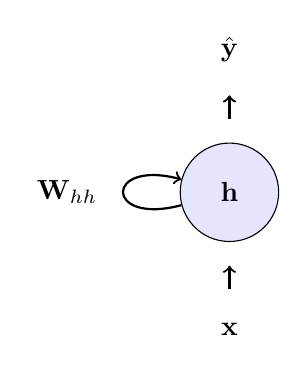
\begin{tikzpicture}[
          neuron/.style={circle, draw, minimum size=1.25cm, inner sep=0pt, fill=blue!10},
          arrow/.style={->, thick},
          node distance=0.9cm
        ]
          \node[neuron] (h) at (0,0) {$\mathbf{h}$};
          \node (x) [below=of h] {$\mathbf{x}$};
          \node (y) [above=of h] {$\hat{\mathbf{y}}$};

          \draw[arrow, shorten >=3mm, shorten <=3mm] (x) -- (h);
          \draw[arrow, shorten >=3mm, shorten <=3mm] (h) -- (y);
          \draw[arrow] (h) edge [loop left, looseness=8] node[left=0.2cm] {$\mathbf{W}_{hh}$} (h);
\end{tikzpicture}


\end{document}
